\documentclass[10pt]{beamer}

\usepackage{bm}

\usepackage{graphicx}

\usepackage{amsmath}
\usepackage{slashed}
\usepackage{hyperref}

\usepackage{booktabs}
\usepackage{subfigure}

\usepackage{amsthm}
\usepackage[utf8x]{inputenc}
\usepackage{color}
\usepackage{cite}
\usepackage{subfigure}
\usepackage{verbatim}
\usepackage{amsfonts}
\usepackage{amssymb}
\usepackage[english]{babel}
\usepackage{graphicx}
\usepackage{textcomp}
\usepackage{Berlin}

\sffamily

\setbeamertemplate{navigation symbols}{}
\setbeamertemplate{bibliography item}[text]
\setbeamertemplate{frametitle continuation}[from second][]
\setbeamertemplate{blocks}[rounded][shadow=true]
\setbeamercovered{transparent}

\setbeamercolor{uppercolor}{fg=white, bg=blue!80!black}
\setbeamercolor{lowercolor}{fg=black, bg=blue!10!white}

\mode
<all>
\newcommand*\oldmacro{}%
\let\oldmacro\insertshorttitle%
\renewcommand*\insertshorttitle{%
  \oldmacro\hfill%
  \insertframenumber\,/\,\inserttotalframenumber} %slides numbering

%%% Title and author
\title{Machine Learning: de la teor\'ia a la pr\'actica}
\subtitle{ {}}
\author[Andr\'es Ram\'irez-Morales]{\textbf{Andr\'es Ram\'irez-Morales}\\ \vspace{5mm} \textbf{e-mail:} andres.ramirez.morales@cern.ch}
%\insertpagenumber
%\begin{document}

\institute{Universidad de Londres}
\date{08-12 de Julio 2019}
	


\begin{document}

\begin{frame}
  
\begin{columns}[T]
\vspace{-3mm}
	\begin{column}{.25\textwidth}
	\begin{figure}
    %\vspace*{7mm}
	
\includegraphics[scale=0.075]{./Figures/atlas.png}
	\end{figure}
	\end{column}
\vspace{-3mm}	    
	\begin{column}{.25\textwidth}	
	\begin{figure}
	
\includegraphics[scale=0.4]{./Figures/QMLogo.jpg}
	\end{figure}
	\end{column}
\vspace{-3mm}		
	\begin{column}{.25\textwidth}	
	\begin{figure}
	
\includegraphics[scale=0.2]{./Figures/conacyt.png}
	\end{figure}
	\end{column}
	
\end{columns} 
  
  \titlepage   
\end{frame}



%\section[]{}
%\begin{frame}
% \tableofcontents
%\end{frame}

\section{Curso}

\subsection{Curso}
\begin{frame}
\frametitle{Lo que este curso es}

\begin{beamerboxesrounded}[upper=uppercolor, lower=lowercolor, shadow=true]{} 

\begin{itemize}
 \item Es una introducci\'on a la programaci\'on cient\'ifica
 \item Pretende dar las herramientas necesarias para que el participante interesado siga aprendiendo
 \item Introducir conceptos de la teor\'ia de Machine Learning
 \item Trabajar con ejemplos simples de Machine Learning
\end{itemize}
\end{beamerboxesrounded}

\end{frame}


\begin{frame}
\frametitle{Lo que este curso NO es}

\begin{beamerboxesrounded}[upper=uppercolor, lower=lowercolor, shadow=true]{} 

\begin{itemize}
 \item Un curso completo de computaci\'on (se requieren un par de a\~nos para dominar el arte)
 \item Un curso de Inteligencia Artificial (solo se toca los puntos claves relacionado a ML)
 \item Un curso de \'algebra y estad\'istica avanzada (se explica la teor\'ia brevemente pero se usar\'an librer\'ias de Python ya establecidas)
\end{itemize}
\end{beamerboxesrounded}

\end{frame}


\begin{frame}
\frametitle{Al finalizar el curso}

\begin{beamerboxesrounded}[upper=uppercolor, lower=lowercolor, shadow=true]{} 

\begin{itemize}
\item El participante tendr\'a una noci\'on consistente de la importancia de la computaci\'on en la ciencia y la tecnolog\'ia 

\item El participante que no ha usado software libre, y su ideolog\'ia, apreciar\'a la importancia del efuerzo global que existe para crear y mantener software libre y \'util para todos

\item Se busca que se tenga una idea clara del poder de la inteligencia artificial en los avances de la tecnolog\'ia y el conocimiento

\end{itemize}
\end{beamerboxesrounded}

\end{frame}


\section{Introducci\'on}

\subsection{Definici\'on}
\begin{frame}
\frametitle{?`Qu\'e es Machine Learning?}

\begin{beamerboxesrounded}[upper=uppercolor, lower=lowercolor, shadow=true]{} 

\begin{itemize}
\item Sabemos que los humanos aprenden de experiencias pasadas
\item Las m\'aquinas siguen las instrucciones dadas por los humanos
\item Imagina que los humanos pueden entrenar m\'aquinas a aprender de experiencias pasadas (datos) y hacer lo que los humanos hacen mucho m\'as r\'apido
\item Hablar de Machine Learning is hablar de Inteligencia Artificial

\end{itemize}
\end{beamerboxesrounded}

\end{frame}

\begin{frame}
\frametitle{?`Qu\'e es Machine Learning?}

\begin{beamerboxesrounded}[upper=uppercolor, lower=lowercolor, shadow=true]{} 

\begin{itemize}
 \item \textbf{Ejemplo}: algoritmo de los vecinos m\'as cercanos
 
\end{itemize}
\end{beamerboxesrounded}

\begin{columns}

\hspace{-7mm}
\begin{column}{.3\textwidth}
\vspace{-3mm}
 \begin{figure}
 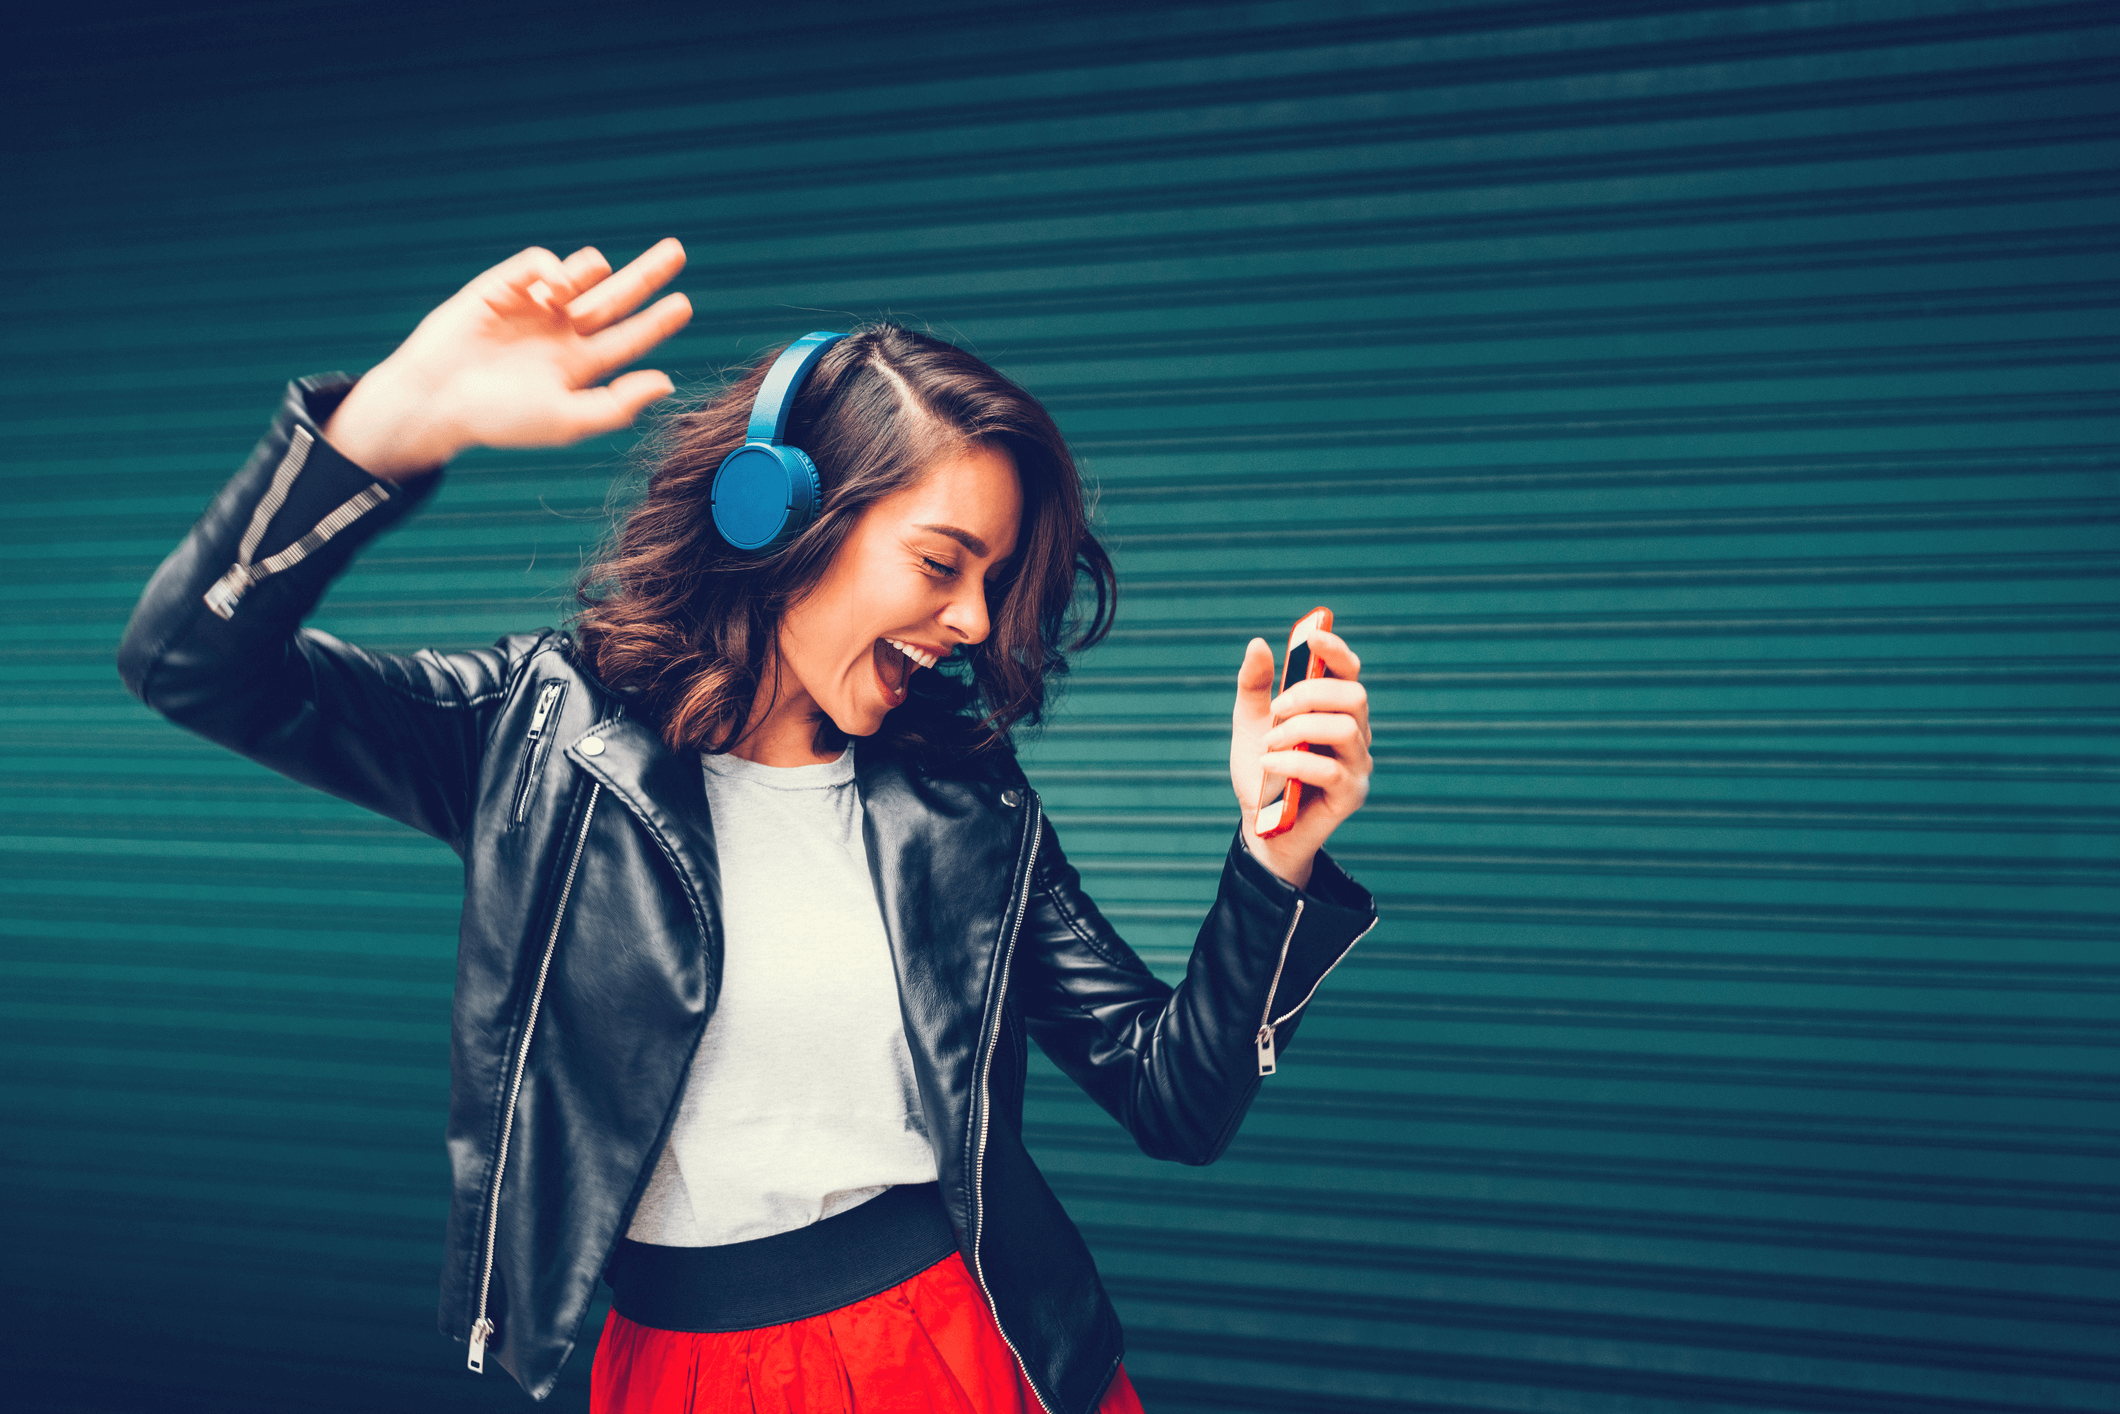
\includegraphics[scale=0.07]{./Figures/music.png} 
 \end{figure}
\end{column}%

\hspace{3mm}
\hspace{3mm}
\begin{column}{.33\textwidth}
\hspace{5mm}
\hspace{5mm}
\vspace{-3mm}
 \begin{figure}
 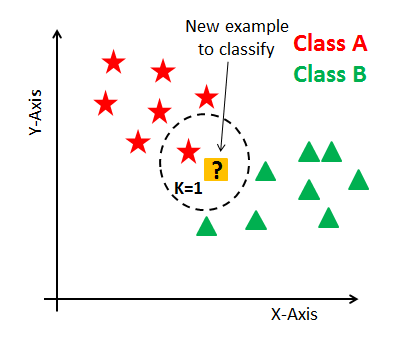
\includegraphics[scale=0.35]{./Figures/nearest.png} 
 \end{figure}  
\end{column}%


\end{columns}
\end{frame}


\section{Instalaci\'on de lo b\'asico}
\subsection{Linux}
\begin{frame}
\frametitle{Instalaci\'on}

\begin{beamerboxesrounded}[upper=uppercolor, lower=lowercolor, shadow=true]{} 

\begin{itemize}
 \item El uso de Linux debe ser una herramienta b\'asica para cualquier cient\'ifico/ingeniero
 \item El uso de Python ha venido mejorando significativamente el desempe\~no de la computaci\'on
\end{itemize}
\end{beamerboxesrounded}

\begin{columns}

\hspace{-7mm}
\begin{column}{.3\textwidth}
\vspace{-3mm}
 \begin{figure}
 
\includegraphics[scale=0.35]{./Figures/ubuntu.png} 
 \end{figure}
\end{column}%

\hspace{3mm}
\hspace{3mm}
\begin{column}{.33\textwidth}
\hspace{5mm}
\hspace{5mm}
\vspace{-3mm}
 \begin{figure}
  
\includegraphics[scale=0.1]{./Figures/python.png} 
 \end{figure}  
\end{column}%

\end{columns}

\end{frame}


\begin{frame}
\frametitle{Instalaci\'on: Hola mundo (Hello world)}

\begin{beamerboxesrounded}[upper=uppercolor, lower=lowercolor, shadow=true]{} 

\begin{itemize}
 \item Uso de python: lenguaje de programaci\'on orientada a objetos
 \item Despu\'es de Hello world, veamos el poder de Python 
 \item Celebremos
\end{itemize}
\end{beamerboxesrounded}

\begin{columns}

\hspace{5mm}
\hspace{5mm}
\begin{column}{\textwidth}
 \begin{figure}
 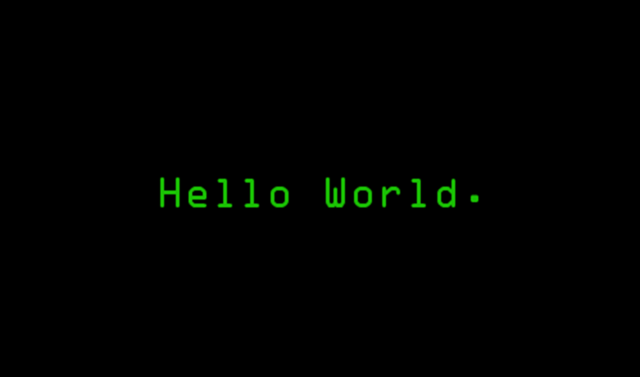
\includegraphics[scale=0.35]{./Figures/hello-world.png} 
 \end{figure}
\end{column}%

\hspace{3mm}
\hspace{3mm}
\begin{column}{.33\textwidth}
\hspace{5mm}
\hspace{5mm}
\vspace{-3mm}
 \begin{figure}
%  
\includegraphics[scale=0.1]{./Figures/python.png} 
 \end{figure}  
\end{column}%

\end{columns}

\end{frame}

\section{ML}
\subsection{ML}

\begin{frame}
\center{Machine Learning}
\end{frame}



\begin{frame}
\frametitle{?`Para qu\'e usar Machine Learning?}

\begin{beamerboxesrounded}[upper=uppercolor, lower=lowercolor, shadow=true]{} 

\begin{itemize}
 \item PayPal, detener estafas: f\'acil de usar, autom\'atico y confiable

\end{itemize}
\end{beamerboxesrounded}

\begin{columns}

\hspace{5mm}
\hspace{5mm}
\begin{column}{\textwidth}
 \begin{figure}
 
\includegraphics[scale=0.35]{./Figures/paypal.png} 
 \end{figure}
\end{column}%

\begin{column}{.33\textwidth}
 \begin{figure}
%  
\includegraphics[scale=0.1]{./Figures/python.png} 
 \end{figure}  
\end{column}%

\end{columns}

\end{frame}


\begin{frame}
\frametitle{Aplicaciones de Machine Learning}
\begin{beamerboxesrounded}[upper=uppercolor, lower=lowercolor, shadow=true]{} 

\begin{itemize}
 \item Buscadores, reconocimiento de voz, reconocimiento de placas, lector de sue\~nos
 \item Machine learning nos facilita la vida, hace los procesos m\'as consistentes y confiables

\end{itemize}
\end{beamerboxesrounded}

\begin{columns}

\hspace{5mm}
\hspace{5mm}
\begin{column}{\textwidth}
 \begin{figure}
 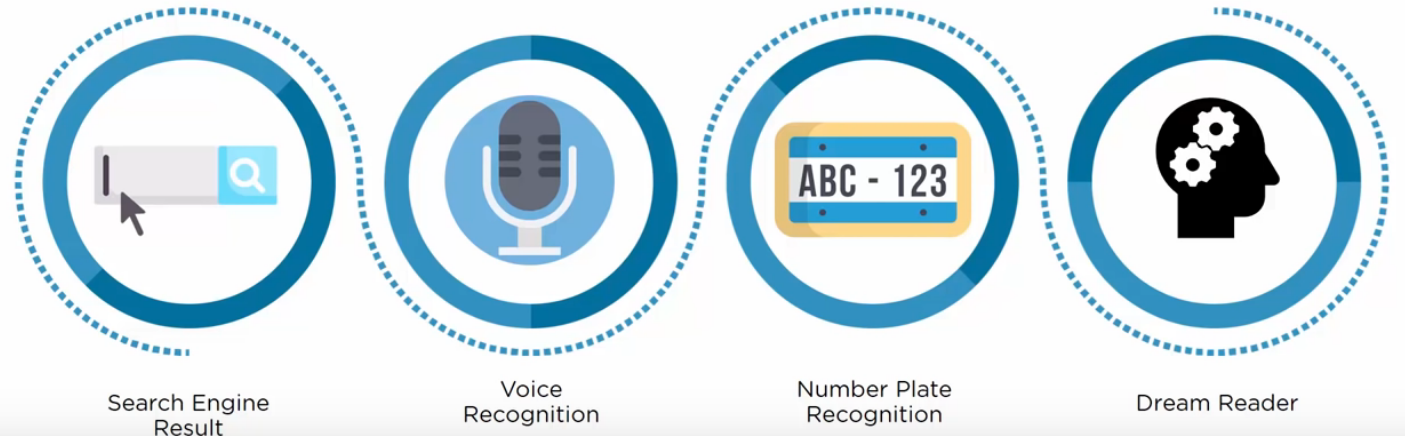
\includegraphics[scale=0.2]{./Figures/aplications.png} 
 \end{figure}
\end{column}%

\begin{column}{.33\textwidth}
 \begin{figure}
%  
\includegraphics[scale=0.1]{./Figures/python.png} 
 \end{figure}  
\end{column}%

\end{columns}

\end{frame}


\begin{frame}
\frametitle{?`C\'omo funciona Machine Learning?}
\begin{beamerboxesrounded}[upper=uppercolor, lower=lowercolor, shadow=true]{} 

\begin{itemize}
 \item Fase 1: \textbf{Aprendizaje}
   \begin{itemize}
     \item Pre-procesamiento: limpiar los datos, darle formato a los datos
     \item Aprender, tomar esos datos y aprender de ellos (supervisado y no supervisado)
     \item Despu\'es de entrenar tu algoritmo, hay que verificar que da las respuestas correctas
   \end{itemize}    
 
 \item Fase 2: \textbf{Predicciones}
   \begin{itemize}
     \item Nuevos datos, model entrenado, predicci\'on, datos predichos
las respuestas correctas
   \end{itemize}    


\end{itemize}
\end{beamerboxesrounded}

\begin{columns}

\hspace{5mm}
\hspace{5mm}
\begin{column}{\textwidth}
 \begin{figure}
 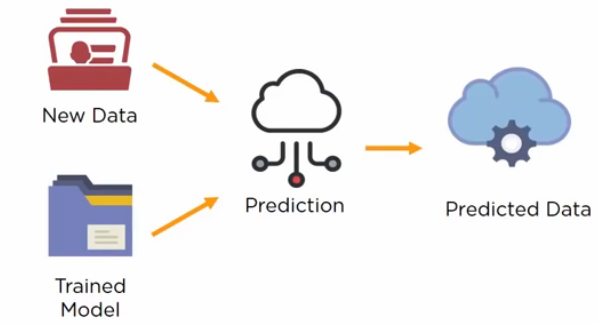
\includegraphics[scale=0.275]{./Figures/fase2.png} 
 \end{figure}
\end{column}%

\begin{column}{.33\textwidth}
 \begin{figure}
%  
\includegraphics[scale=0.1]{./Figures/python.png} 
 \end{figure}  
\end{column}%

\end{columns}

\end{frame}



\begin{frame}
\frametitle{Tipos de Machine Learning}
\begin{beamerboxesrounded}[upper=uppercolor, lower=lowercolor, shadow=true]{} 

\begin{itemize}
 \item Aprendizaje supervisado
 \item Aprendizaje NO supervisado
 \item Aprendizaje reforzado
\end{itemize}
\end{beamerboxesrounded}

\begin{columns}

\hspace{5mm}
\hspace{5mm}
\begin{column}{\textwidth}
 \begin{figure}
 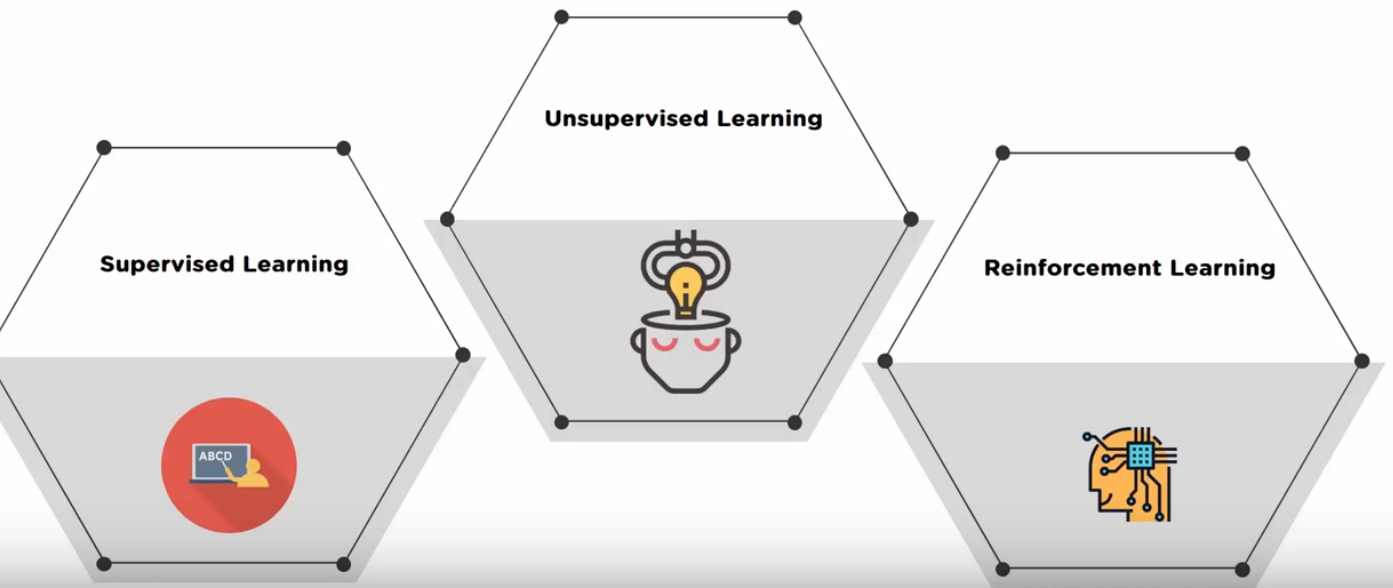
\includegraphics[scale=0.175]{./Figures/tipos.png} 
 \end{figure}
\end{column}%

\begin{column}{.33\textwidth}
 \begin{figure}
%  
\includegraphics[scale=0.1]{./Figures/python.png} 
 \end{figure}  
\end{column}%

\end{columns}

\end{frame}


\begin{frame}
\frametitle{Aprendizaje supervisado}
\begin{beamerboxesrounded}[upper=uppercolor, lower=lowercolor, shadow=true]{} 

\begin{itemize}
 \item El modelo de Machine Learning aprende de datos insertados en el pasado y hace futuras predicciones como salida
 \item \textbf{Tipos de Aprendizaje supervisado} 
 \begin{itemize}
   \item Clasificaci\'on: separar datos en diferentes tipos, (\'arboles de decisi\'on o support vector machine)
   \item Regresi\'on: basado en datos anteriores, la m\'aquina predice un continuo de valores (regresi\'on lineal, regresi\'on polinomial)
 \end{itemize}
  
\end{itemize}
\end{beamerboxesrounded}

\begin{columns}

\hspace{5mm}
\hspace{5mm}
\begin{column}{\textwidth}
 \begin{figure}
 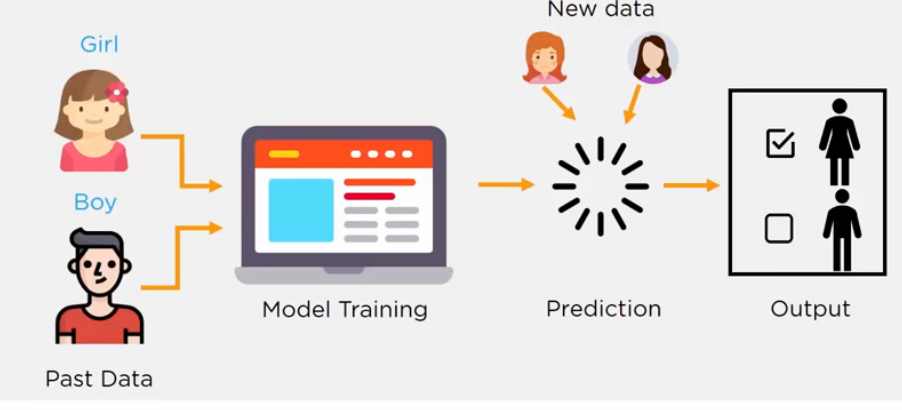
\includegraphics[scale=0.2]{./Figures/clasificacion.png} 
 \end{figure}
\end{column}%

\begin{column}{.33\textwidth}
 \begin{figure}
%  
\includegraphics[scale=0.1]{./Figures/python.png} 
 \end{figure}  
\end{column}%

\end{columns}

\end{frame}


\begin{frame}
\frametitle{Aprendizaje supervisado: Regresi\'on lineal}
\begin{beamerboxesrounded}[upper=uppercolor, lower=lowercolor, shadow=true]{} 

\begin{itemize}
 \item El precio de una casa depende del tama\~no
 \item Usar los datos anteriores para predecir el precio de una casa de cualquiero tama\~no
  
\end{itemize}
\end{beamerboxesrounded}

\begin{columns}

\hspace{5mm}
\hspace{5mm}
\begin{column}{\textwidth}
 \begin{figure}
 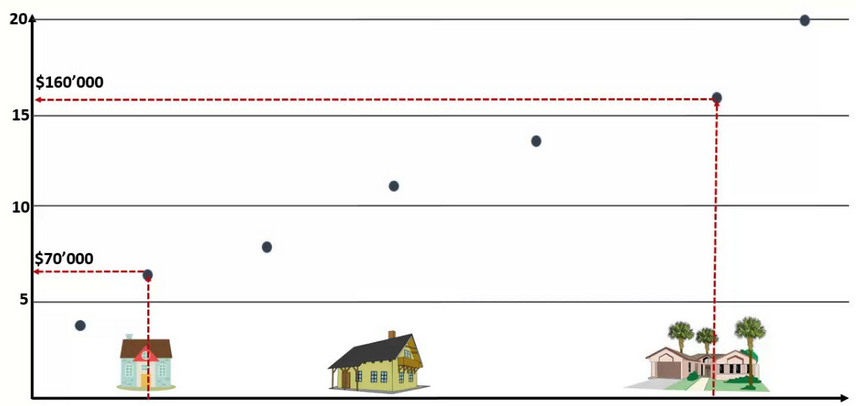
\includegraphics[scale=0.3]{./Figures/linear.png} 
 \end{figure}
\end{column}%

\begin{column}{.33\textwidth}
 \begin{figure}
%  
\includegraphics[scale=0.1]{./Figures/python.png} 
 \end{figure}  
\end{column}%

\end{columns}

\end{frame}


\begin{frame}
\frametitle{Aprendizaje NO supervisado}
\begin{beamerboxesrounded}[upper=uppercolor, lower=lowercolor, shadow=true]{} 

\begin{itemize}
 \item Significa que la m\'aquina aprende utilizando datos insertados sin etiquetar
 \item Permite que el algoritmo actue sobre los datos sin ninguna gu\'ia
 \item Recordemos que para el caso de aprendizaje supervisado, ten\'iamos una respuesta, aqu\'i no la tenemos, es decir permitimos que el algoritmo obtenga las respuestas para nosotros
 \item \textbf{Tipos de Aprendizaje NO supervisado} 
 \begin{itemize}
   \item Clustering: Es usado para analizar y agrupar datos (k-means, clustering de jerarqu\'ia, modelo escondido de Markov)
   \item Asociaci\'on: descubre la posibilidad de la ocurrencia asociada  en una colecci\'on de objetos (Algoritmo Apriori, y crecimiento-FP)
 \end{itemize}
  
\end{itemize}
\end{beamerboxesrounded}

\begin{columns}

\hspace{5mm}
\hspace{5mm}
\begin{column}{\textwidth}
 \begin{figure}
 %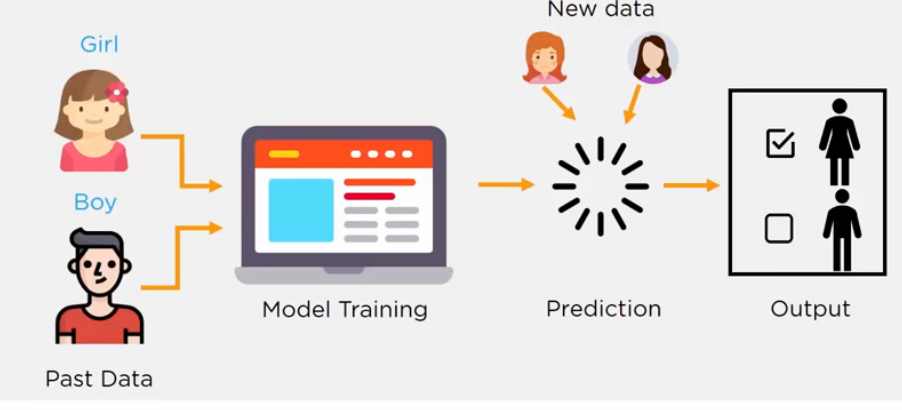
\includegraphics[scale=0.2]{./Figures/clasificacion.png} 
 \end{figure}
\end{column}%

\begin{column}{.33\textwidth}
 \begin{figure}
%  
\includegraphics[scale=0.1]{./Figures/python.png} 
 \end{figure}  
\end{column}%

\end{columns}

\end{frame}


\begin{frame}
\frametitle{Aprendizaje NO supervisado: k-means clustering}
\begin{beamerboxesrounded}[upper=uppercolor, lower=lowercolor, shadow=true]{} 

\begin{itemize}
 \item La idea es tomar varios similares objetos y clasificarlos en clusters
   
\end{itemize}
\end{beamerboxesrounded}

\begin{columns}

\hspace{5mm}
\hspace{5mm}
\begin{column}{\textwidth}
 \begin{figure}
 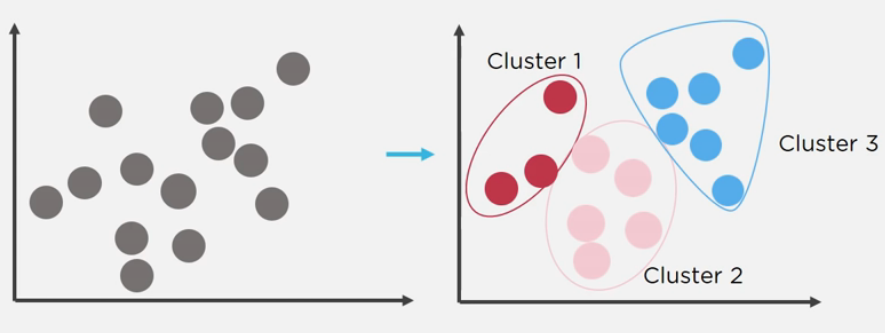
\includegraphics[scale=0.35]{./Figures/cluster.png} 
 \end{figure}
\end{column}%

\begin{column}{.33\textwidth}
 \begin{figure}
%  
\includegraphics[scale=0.1]{./Figures/python.png} 
 \end{figure}  
\end{column}%

\end{columns}

\end{frame}


\begin{frame}
\frametitle{Aprendizaje NO supervisado: k-means clustering}
\begin{beamerboxesrounded}[upper=uppercolor, lower=lowercolor, shadow=true]{} 

\begin{itemize}
 \item \textbf{Paso 1:} Iniciar aleatoriamente dos puntos llamados centroides
 \item \textbf{Paso 2:} Basado en la distancia de los centros se har\'a un grupo
 \item \textbf{Paso 3:} Mover los centroides un poco para ajustarlos para optimizar, repetir esto hasta que los centroides dejen de cambiar de posici\'on, es decir que los grupos esten bien definidos (convergencia) 
   
\end{itemize}
\end{beamerboxesrounded}

\begin{columns}
\begin{column}{.5\textwidth}
 \begin{figure}
 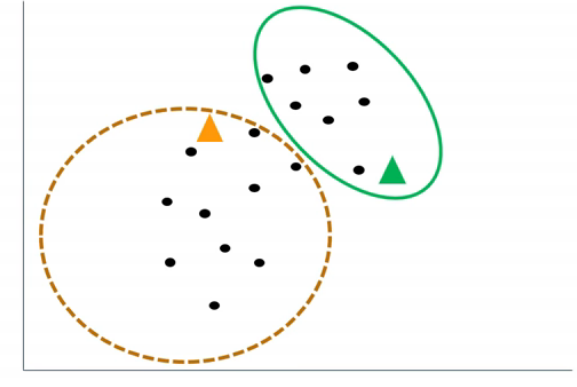
\includegraphics[scale=0.25]{./Figures/centroids.png} 
 \end{figure}
\end{column}%

\begin{column}{.5\textwidth}
 \begin{figure}
 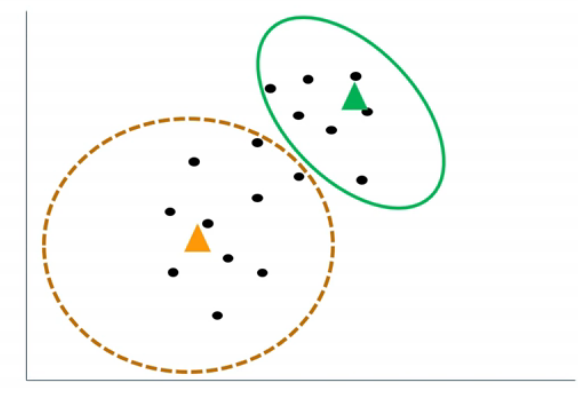
\includegraphics[scale=0.25]{./Figures/centroids_static.png} 
 \end{figure}  
\end{column}%

\end{columns}

\end{frame}



\begin{frame}
\frametitle{k-means clustering: An\'alisis del clima}
\begin{beamerboxesrounded}[upper=uppercolor, lower=lowercolor, shadow=true]{} 

\begin{itemize}
 \item \textbf{Problema:} predecir el clima usando Machine Learning
 \item \textbf{Posibles retos:}
   \begin{itemize}
     \item Identificar las \'areas donde hay lluvia
     \item Considerar la temperatura y la presi\'on como par\'ametros: el algoritmo k-means indetificar\'a las regiones que est\'an expuestas a fuerte lluvia 
   \end{itemize}
    
\end{itemize}
\end{beamerboxesrounded}

%\begin{columns}
%\begin{column}{.5\textwidth}
% \begin{figure}
% 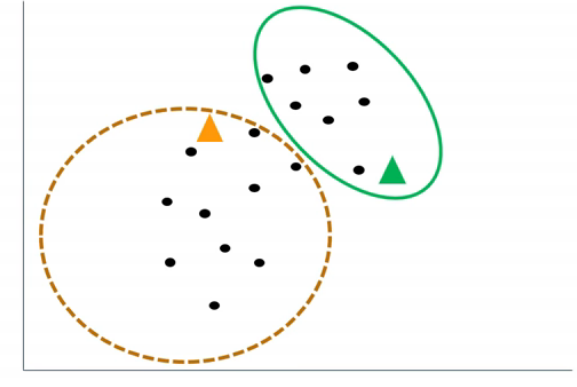
\includegraphics[scale=0.25]{./Figures/centroids.png} 
% \end{figure}
%\end{column}%
%
%\begin{column}{.5\textwidth}
% \begin{figure}
% 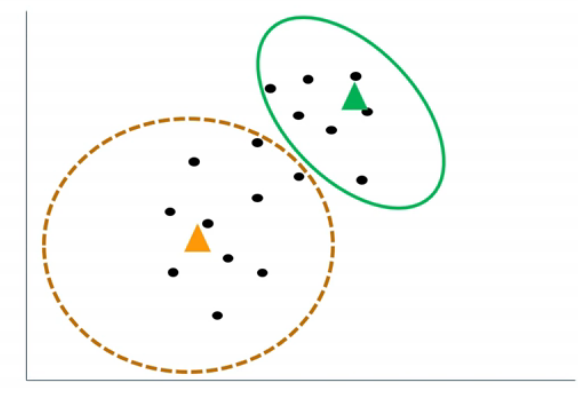
\includegraphics[scale=0.25]{./Figures/centroids_static.png} 
% \end{figure}  
%\end{column}%
%
%\end{columns}
\end{frame}



\begin{frame}
\frametitle{k-means clustering: Comprimir una imagen}
\begin{beamerboxesrounded}[upper=uppercolor, lower=lowercolor, shadow=true]{} 

\begin{itemize}
 \item \textbf{Problema:} comprimir una imagen usando Machine Learning
 \item \textbf{Posibles retos:}
   \begin{itemize}
     \item Identificar las colores principales que representen a la imagen
     \item Mapear los colores 24-bit a una dimensi\'on m\'as baja usando asignaci\'on de clusters 
   \end{itemize}
    
\end{itemize}
\end{beamerboxesrounded}

\begin{columns}
\begin{column}{.5\textwidth}
 \begin{figure}
 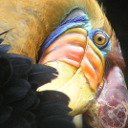
\includegraphics[scale=0.75]{./Figures/bird_small.png} 
 \end{figure}
\end{column}%

%\begin{column}{.5\textwidth}
% \begin{figure}
% 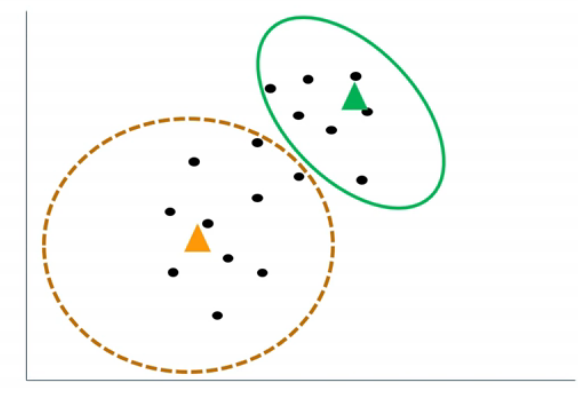
\includegraphics[scale=0.25]{./Figures/centroids_static.png} 
% \end{figure}  
%\end{column}%
\end{columns}
\end{frame}


\section{Neural Networks}

\subsection{Neural Networks}
\begin{frame}
Neural Networks
\end{frame}


\begin{frame}
\frametitle{Neural Networks}

\begin{columns}
\begin{column}{.5\textwidth}
\begin{beamerboxesrounded}[upper=uppercolor, lower=lowercolor, shadow=true]{} 

\begin{itemize}
 \item \textbf{Problema:} identificar un numero tres manuscrito con una computadora
 \item \textbf{Posibles retos}
   \begin{itemize}
     \item Tu cerebro no tiene problema alguno para reconocerlo como un tres
     \item La luz que llega de estos tres's es muy diferente pero algo en nuestra inteligente corteza cerebral los identifica como (la misma idea) tres's apesar de que el acomodo de sus pixeles es muy diferente
     
   \end{itemize}
    
\end{itemize}
\end{beamerboxesrounded}


\end{column}%

\begin{column}{.5\textwidth}
 \begin{figure}
 \vspace{-10mm}
 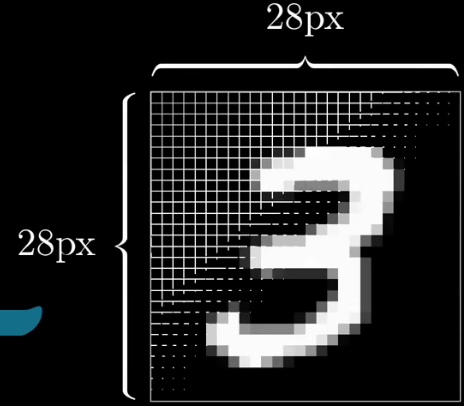
\includegraphics[scale=0.15]{./Figures/tres_pixel.png}
 \hspace{10mm}
 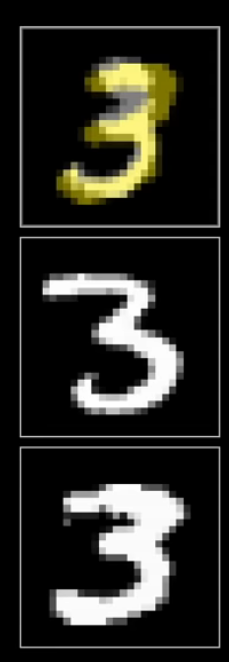
\includegraphics[scale=0.2]{./Figures/tres_pixel_2.png}  
 \end{figure}  
\end{column}%
\end{columns}

\end{frame}


\begin{frame}
\frametitle{Neural Networks}
\begin{beamerboxesrounded}[upper=uppercolor, lower=lowercolor, shadow=true]{} 

\begin{itemize}
 \item Al mismo tiempo reconoce otras im\'agenes como otras ideas
    
\end{itemize}
\end{beamerboxesrounded}

\begin{columns}
\begin{column}{.5\textwidth}
 \begin{figure}
 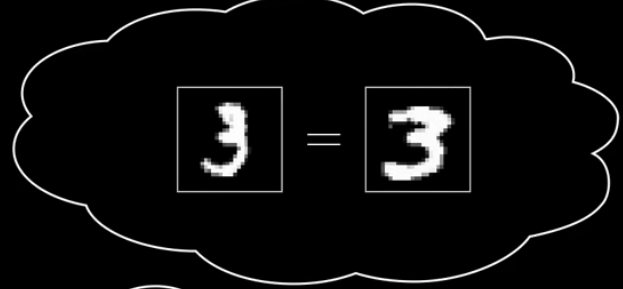
\includegraphics[scale=0.2]{./Figures/tres_igual.png}
 \end{figure}  
\end{column}%

\begin{column}{.5\textwidth}
 \begin{figure}
 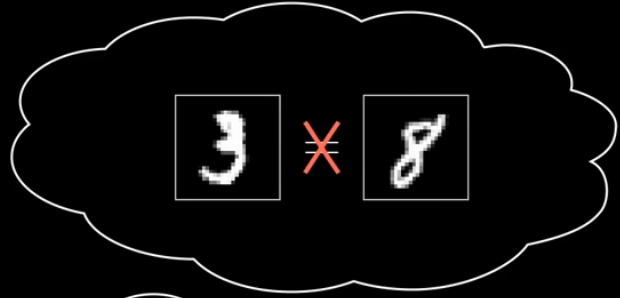
\includegraphics[scale=0.2]{./Figures/tres_ocho.png}  
 \end{figure}  
\end{column}%
\end{columns}

\end{frame}

\begin{frame}
\frametitle{Neural Networks}
\begin{beamerboxesrounded}[upper=uppercolor, lower=lowercolor, shadow=true]{} 

\begin{itemize}
 \item Escribir un programa que tome una red de $28\times 28$ pixeles y que de una buena suposici\'on de que n\'umero se trata
 \item \textbf{Soluci\'on} Neural Networks
    
\end{itemize}
\end{beamerboxesrounded}

\begin{columns}
\begin{column}{\textwidth}
 \begin{figure}
 \begin{center}
 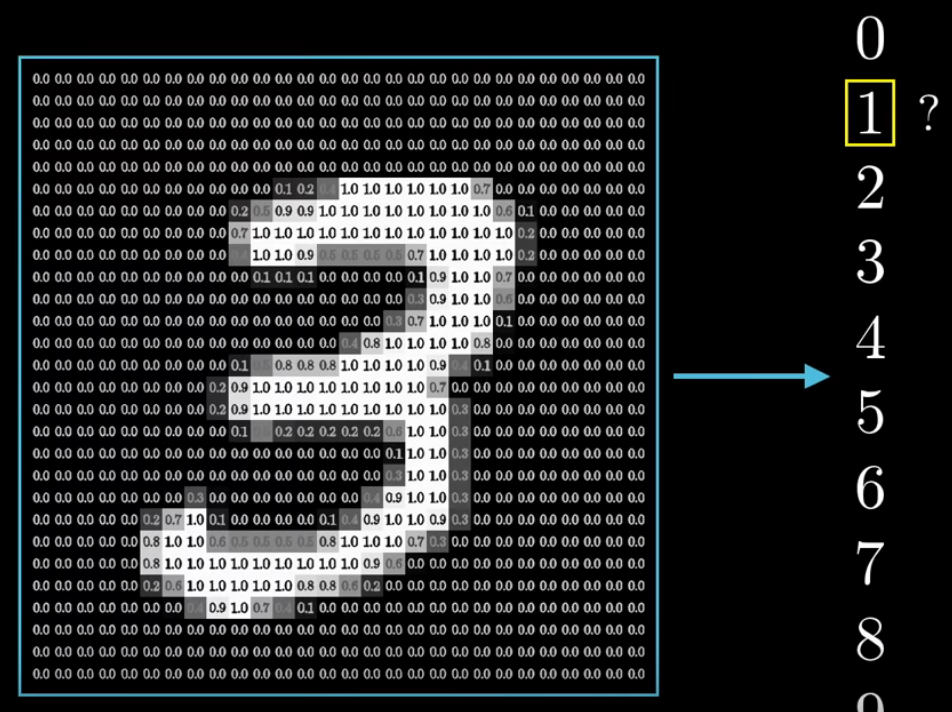
\includegraphics[scale=0.2]{./Figures/tres_grid.png} 
 \end{center}
 \end{figure}  
\end{column}%

%\begin{column}{.5\textwidth}
% \begin{figure}
% 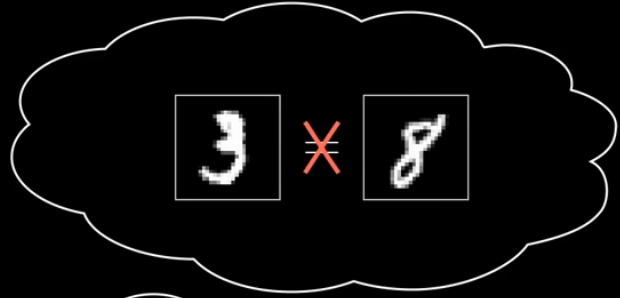
\includegraphics[scale=0.2]{./Figures/tres_ocho.png}  
% \end{figure}  
%\end{column}%
\end{columns}

\end{frame}


\begin{frame}
\frametitle{?`Qu\'e es una Neural Network?}
\begin{beamerboxesrounded}[upper=uppercolor, lower=lowercolor, shadow=true]{} 

\begin{itemize}
 \item  Neural Networks se expresan matem\'aticamente:
 \begin{equation*}
  a_{l+1} = \sigma(W_l a_l + b_l)
 \end{equation*}
 
\end{itemize}
\end{beamerboxesrounded}

\begin{columns}
\begin{column}{.5\textwidth}
 \begin{figure}
  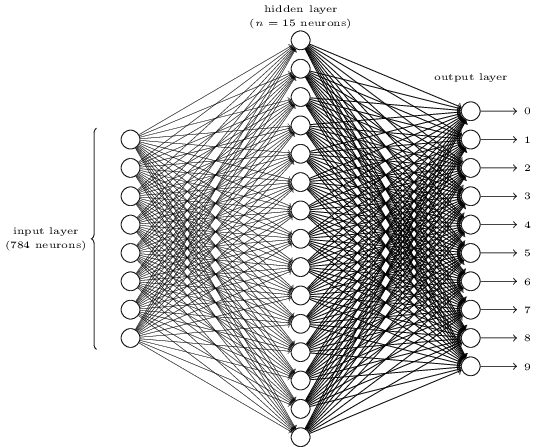
\includegraphics[scale=0.275]{./Figures/NeuralNetwork_big.png}
 \end{figure}  
\end{column}%

\begin{column}{.5\textwidth}
 \begin{figure}
  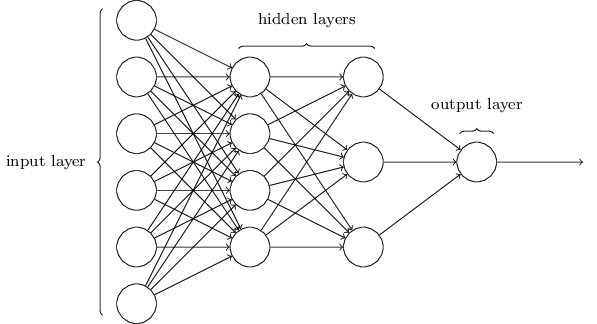
\includegraphics[scale=0.275]{./Figures/NeuralNetwork_small.png}
 \end{figure}  
\end{column}%

\end{columns}

\end{frame}


\begin{frame}
\frametitle{?`Qu\'e es una Neural Network?}
\begin{beamerboxesrounded}[upper=uppercolor, lower=lowercolor, shadow=true]{} 

\begin{itemize}
 \item  Percepci\'on multicapa, esta es la forma m\'as simple de NN, pero a\'un as\'i puede aprender a reconocer n\'umeros manuscritos 
  
\end{itemize}
\end{beamerboxesrounded}

\begin{columns}
\begin{column}{.5\textwidth}
 \begin{figure}
 \begin{center}
  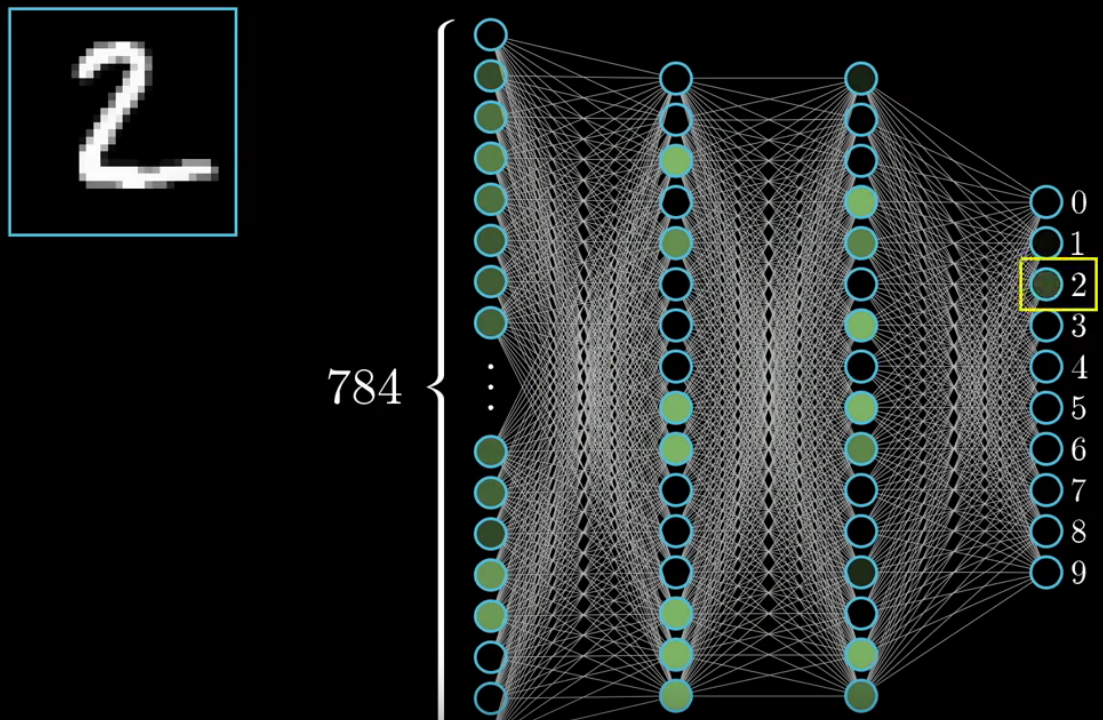
\includegraphics[scale=0.175]{./Figures/dos_NN.png} 
 \end{center}
 \end{figure}  
\end{column}%

%\begin{column}{.5\textwidth}
% \begin{figure}
%  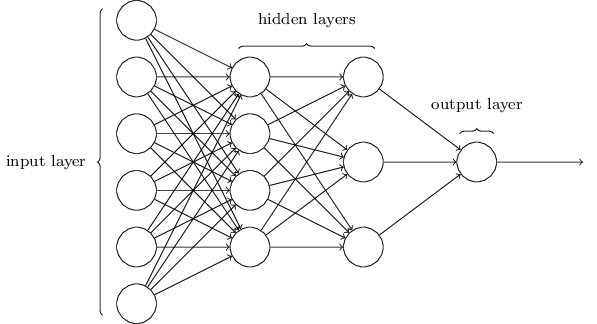
\includegraphics[scale=0.275]{./Figures/NeuralNetwork_small.png}
% \end{figure}  
%\end{column}%

\end{columns}
\end{frame}


\begin{frame}
\frametitle{?`Qu\'e es una Neural Network?}
\begin{beamerboxesrounded}[upper=uppercolor, lower=lowercolor, shadow=true]{} 

\begin{itemize}
 \item  Est\'a inspirada por el cerebro:
 \begin{itemize}
  \item \textbf{Neural:} ?`Cu\'ales son las neuronas? 
  \centerline{Neurona: algo que guarda un n\'umero entre 0 y 1:}
  \centerline{\textbf{ n\'umero de activaci\'on}}
    \item \textbf{Networks (redes):} ?`En qu\'e sentido est\'an conectadas?
 \end{itemize}  
  
\end{itemize}
\end{beamerboxesrounded}

\begin{columns}
 \hspace*{-10mm}
 \hspace*{-10mm}

\begin{column}{.5\textwidth}
 \begin{figure}
 \begin{center}
  
\includegraphics[scale=0.125]{./Figures/brain.jpg} 
 \end{center}
 \end{figure}  
\end{column}%

\begin{column}{.5\textwidth}
\vspace{-3.5mm}
\vspace{-3.5mm}
 \begin{figure}
  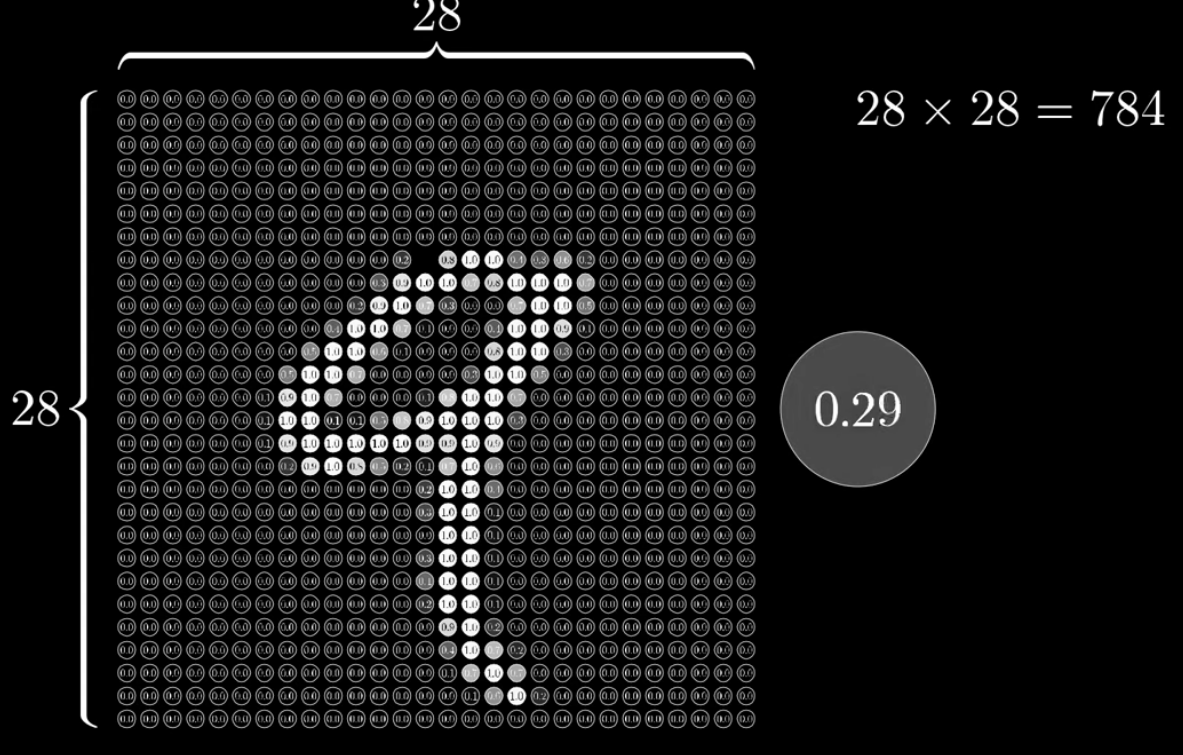
\includegraphics[scale=0.155]{./Figures/neurona_number.png}
 \end{figure}  
\end{column}%

\end{columns}

\end{frame}



\begin{frame}
\frametitle{?`Qu\'e es una Neural Network?}
\begin{beamerboxesrounded}[upper=uppercolor, lower=lowercolor, shadow=true]{} 

\begin{itemize}
\item Cada pixel de la imagen anterior representa una neurona de la primera capa de la red de neuronas

\item La \'ultima capa tiene 10 neuronas que representan cada digito, la activaci\'on en estas neuronas representa que tanto el sistema piensa que una imagen dada corresponde a un digito dado

\item La forma en que la red opera es que los n\'umero de activaci\'on en una capa determina la activaci\'on de la siguiente capa: el coraz\'on del m\'etodo es el mecanismo de procesamiento de como estos n\'umeros de activaci\'on activan a los de la siguiente capa (parecido a nuestro cerebro)

\item La red que vamos a trabajar ya ha sido entrenada de como reconocer digitos: si se inserta una imagen (784 neuronas) y siguiendo los pixeles en la imagen ese patr\'on de activaciones cuasa activaciones muy espec\'ificas en las siguientes capa hasta llegar a la capa final y la neurona m\'as brillante nos dice que digito esta imagen representa  

 
\end{itemize}
\end{beamerboxesrounded}

\end{frame}


\begin{frame}
\frametitle{?`Qu\'e es una Neural Network?}
\begin{beamerboxesrounded}[upper=uppercolor, lower=lowercolor, shadow=true]{} 

\begin{itemize}
\item ?`Por qu\'e estructura de capas y por qu\'e se comporta inteligente?
\item Nuestro ojo reconoce \'ovalos y palitos, esperar\'iamos que cada neurona de la segunda a la \'ultima capa, corresponda con cada una de estas subcomponentes 
\item Requiere aprender que combinaci\'on de subcomponentes corresponde a que digito
\item Reconocer un \'ovalo, reconocer los peque\~nos bordes
\item No solo reconocimiento de imagen, si no discurso de personas: entra audio crudo y el sonido se descompone en palabras y las palabras en letras 

\end{itemize}
\end{beamerboxesrounded}


\end{frame}


\begin{frame}
\frametitle{?`Qu\'e es una Neural Network?}
\begin{beamerboxesrounded}[upper=uppercolor, lower=lowercolor, shadow=true]{} 

\begin{itemize}
\item Como las activaciones en una capa podr\'ian determinar la activacion de las siguientes un mecanismo que:\\
\begin{center}
\mbox{pixels$\rightarrow$bordes$\rightarrow$patrones$\rightarrow$digitos}
\end{center}
 
\end{itemize}
\end{beamerboxesrounded}

\begin{columns}
\begin{column}{.5\textwidth}
  \begin{figure}
  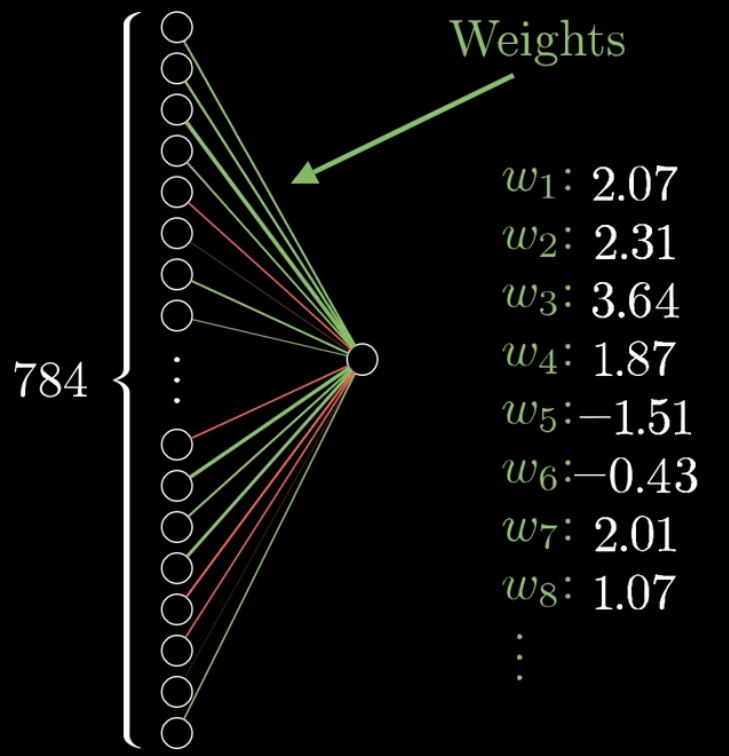
\includegraphics[scale=0.155]{./Figures/weights.png}
 \end{figure}  
\end{column}%

\begin{column}{.5\textwidth}
Obtener la suma ponderada de los n\'umeros de activaci\'on
\begin{equation*}
w_1 a_1+w_2 a_2+w_3 a_3+...+w_n a_n
\end{equation*}
Queremos que las activaciones [0,1], apretar la suma un n\'umero no cualquiera



\end{column}%
\end{columns}
\end{frame}



\begin{frame}
\frametitle{?`Qu\'e es una Neural Network?}

\begin{columns}
\begin{column}{\textwidth}
  \begin{figure}
  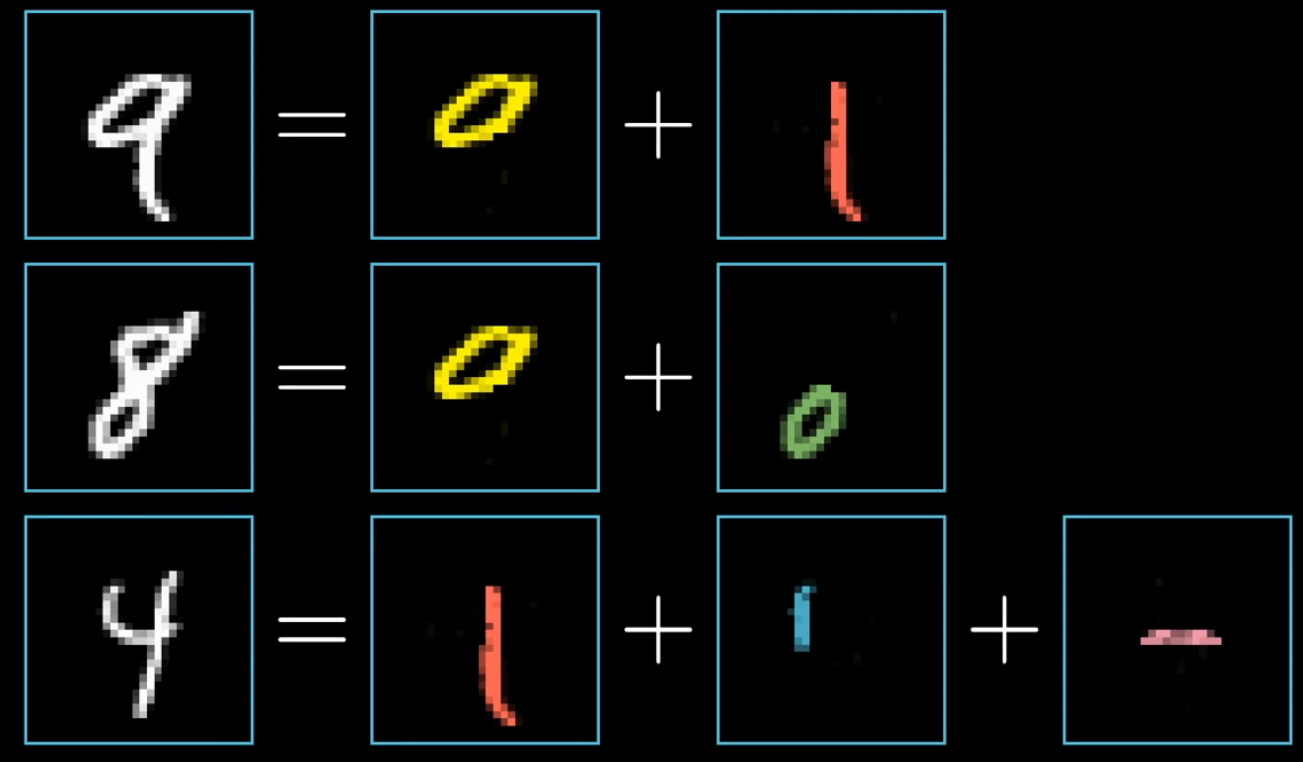
\includegraphics[scale=0.155]{./Figures/descomp_num.png}
 \end{figure}  
\end{column}%
\end{columns}
\end{frame}



\begin{frame}
\frametitle{?`Qu\'e es una Neural Network?}
\begin{beamerboxesrounded}[upper=uppercolor, lower=lowercolor, shadow=true]{} 

\begin{itemize}
\item Usamos la funci\'on Sigmoid:
\begin{equation*}
\sigma(w_1 a_1+w_2 a_2+w_3 a_3+...+w_n a_n)
\end{equation*}

\item La activaci\'on de la neurona es la medida de que tan positiva es la suma ponderada 
\item Se necesita una adici\'on para la inactividad, $i.e.$ quiz\'a  no interesa la neurona activa arriba de cero, $>10$
\begin{equation*}
\sigma(w_1 a_1+w_2 a_2+w_3 a_3+...+w_n a_n-10)
\end{equation*}

 
\end{itemize}
\end{beamerboxesrounded}

\end{frame}



\begin{frame}
\frametitle{?`Qu\'e es una Neural Network?} 
  \begin{figure}
  \includegraphics[scale=0.25]{./Figures/sigmoid.png}
  \end{figure}
\end{frame}



\begin{frame}
\frametitle{?`Qu\'e es una Neural Network?}
\begin{beamerboxesrounded}[upper=uppercolor, lower=lowercolor, shadow=true]{} 

\begin{itemize}
\item Los pesos (weights) dicen que patr\'on de pixeles esta neurona en la segunda capa esta siguiendo y la adici\'on dice que tan grande la suma ponderada necesita ser antes de que las neuronas empiecen a ser significativamente activas

\item Cuando hablamos de aprendizaje estamos hablando de encontrar los pesos y las adiciones para esta gran cantidad de n\'umeros para que resulvan el problema 
 \end{itemize}

\begin{equation*}
a_0^1 = \sigma(w_{0,0} a_0^{(0)} + w_{0,1} a_1^{(0)} +...+ w_{0,n} a_n^{(0)}+b_0)
\end{equation*}
 
\end{beamerboxesrounded}

\end{frame}



\begin{frame}
\frametitle{?`Qu\'e es una Neural Network?}
\begin{beamerboxesrounded}[upper=uppercolor, lower=lowercolor, shadow=true]{} 

\begin{itemize}
\item Representaci\'on matricial 

\begin{equation*}
\sigma (
\begin{pmatrix}
w_{0,0} & w_{0,1} & . \quad . \quad . \quad & w_{0,n} \\
\\
w_{1,0} & w_{1,1} & . \quad . \quad . \quad & w_{1,n} \\
. \\
. \\
. \\
w_{k,0} & w_{k,1} & . \quad . \quad . \quad & w_{k,n} \\
\end{pmatrix}
\begin{pmatrix}
a_{0}^{(0)} \\
\\
a_{1}^{(0)} \\
. \\
. \\
. \\
a_{n}^{(0)} 
\end{pmatrix}
\: + \:
\begin{pmatrix}
b_{0}^{(0)} \\
\\
b_{1}^{(0)} \\
. \\
. \\
. \\
b_{n}^{(0)} 
\end{pmatrix}
) 
\end{equation*}

\item En forma compacta la transici\'on de una capa a la que sigue:
\begin{equation*}
\mathbf{a}^{(1)}=\sigma(\mathbf{Wa}^{(0)}+\mathbf{b})
\end{equation*}

\item Mejor pensamos que una neurona es m\'as bien una funci\'on (la red entera es una funci\'on, muy complicada con muchos par\'ametros1)
\end{itemize} 

\end{beamerboxesrounded}


\end{frame}





%\section{Recapitulaci\'on}
%\subsection{Recapitulaci\'on}
\begin{frame}
\frametitle{Recapitulaci\'on}

\begin{beamerboxesrounded}[upper=uppercolor, lower=lowercolor, shadow=true]{} 

\begin{itemize}

\item Se introdujo el concepto de Machine Learning
\item Se revis\'o la importancia del uso de Machine Learning en la ciencia e ingienier\'ia

\end{itemize}
\end{beamerboxesrounded}

\end{frame}



\begin{frame}
\centering{PREGUNTAS}
\end{frame}



%\begin{frame}
%
%\frametitle{BackUp}
%
% \begin{figure}
%% \scriptsize{Proton}
% \includegraphics[scale=0.175]{./Figures/MODELO.png}
% \end{figure}  
%
%\end{frame}



\end{document}